\documentclass[../opis-rozwiazania.tex]{subfiles}

\begin{document}
\label{communication-sec}

\subsection{Utworzenie sesji}

Celem tej sekwencji komunikacji jest odnalezienie istniejącej już sesji lub stworzenie nowej.
Zakładamy, że w systemie zawsze jest jakaś wolna maszyna.
Inaczej zgłaszamy użytkownikowi błąd.

\begin{figure}[H]
  \centering
  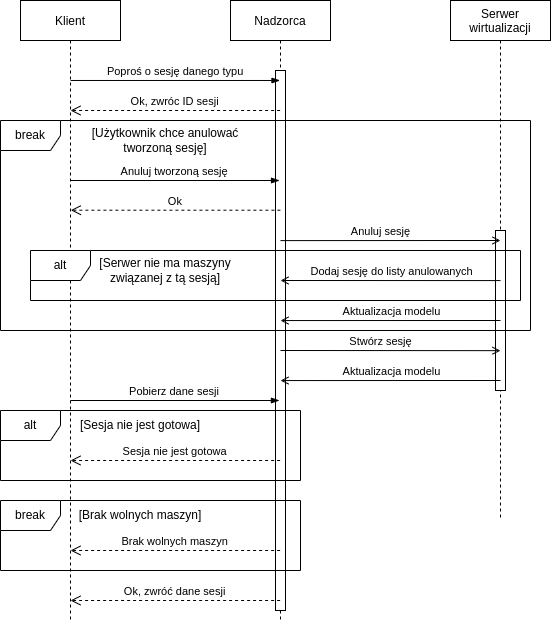
\includegraphics[width=0.8\textwidth]{../diagrams/sequence_diagrams/tworzenie_sesji.png}
  \caption{Sekwencja komunikacji utworzenia sesji}
  \label{figure:diagrams:sequence_diagrams:tworzenie_sesji}
\end{figure}

Po prośbie użytkownika nadzorca znajduje wolną maszynę i prosi konkretny serwer wirtualizacji, aby spróbował utworzyć sesje dla pewnego użytkownika.
Gdy to się uda, ten wysyła zbiorczą kolejką do nadzorców informacje o zmianie modelu.
W przeciwnym przypadku nadzorca powtarza wyszukanie wolnej maszyny.
Czy nadzorca musi powtórzyć wyszukiwanie decyduje stan otrzymanej maszyny (m.in. czy sesja do niej przypisana należy do tego użytkownika).

Może się zdarzyć także anulowanie wyszukiwania przez użytkownika.
Wtedy, jeżeli maszyna jest już przydzielona użytkownikowi, to serwer wirtualizacji jest powiadamiany o anulowaniu sesji.
Jeżeli nie została jeszcze utworzona, to nadzorca dopilnuje aby więcej nie szukać sesji lub wyłączy ją w miarę potrzeby.

\subsection{Zakończenie sesji}

Sekwencja ta zainicjowana jest poprzez utracenie połączenia z użytkownikiem maszyny.
Serwer powiadamia o tym fakcie nadzorców, po czym oczekuje na polecenie wyłączenia maszyny przesłane przez nadzorcę. Serwer może odmówić z powodu różnic modelu, lub jeżeli maszyna znów jest używana przez użytkownika, ignorując wiadomość.

\begin{figure}[H]
  \centering
  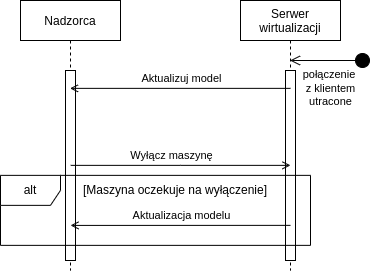
\includegraphics[width=0.6\textwidth]{../diagrams/sequence_diagrams/konczenie_sesji.png}
  \caption{Sekwencja komunikacji zakończenia sesji}
  \label{figure:diagrams:sequence_diagrams:konczenie_sesji}
\end{figure}

\subsection{Aktualizacja stanu}

Nadzorca może w każdej chwili poprosić wszystkie serwery wirtualizacji
o przesłanie ich aktualnego stanu poprzez wspólna kolejkę do serwerów wirtualizacji (rozdział \ref{modules:broker}, kolejka \ref{modules:broker:queue-virtsrv}).
Serwery muszą bezwarunkowo odpowiedzieć aktualnym stanem do wspólnej kolejki zwrotnej (rozdział \ref{modules:broker}, kolejka \ref{modules:broker:queue-overseers}).

\begin{figure}[H]
  \centering
  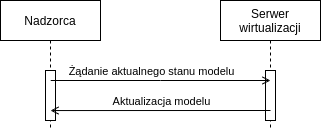
\includegraphics[width=0.6\textwidth]{../diagrams/sequence_diagrams/aktualizacja_stanu.png}
  \caption{Sekwencja komunikacji aktualizacji stanu systemu}
  \label{figure:diagrams:sequence_diagrams:aktualizacja_stanu}
\end{figure}

\subsection{Włączenie maszyny}

Nadzorca może poprosić konkretny serwer wirtualizacji, aby utworzył maszynę o konkretnej nazwie.
Jeżeli maszynie nie istnieje, to zostanie ona uruchomiona oraz serwer odeśle powiadomienie zbiorcza kolejką (rozdział \ref{modules:broker}, kolejka \ref{modules:broker:queue-overseers}) o zmianie modelu.
W przeciwnym wypadku nie zrobi nic.

\begin{figure}[H]
  \centering
  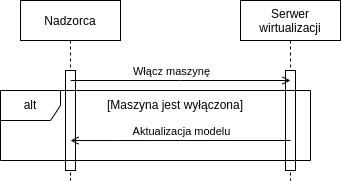
\includegraphics[width=0.6\textwidth]{../diagrams/sequence_diagrams/wlaczenie_maszyny.png}
  \caption{Sekwencja komunikacji włączenia maszyny}
  \label{figure:diagrams:sequence_diagrams:wlaczenie_maszyny}
\end{figure}

\subsection{Wyłączenie maszyny}

Nadzorca może poprosić konkretny serwer wirtualizacji, aby wyłączył konkretną maszynę wirtualną.
Jeżeli maszynę można wyłączyć to zostanie ona wyłączona.
Następnie serwer wirtualizacji odeśle powiadomienie zbiorczą kolejką (rozdział \ref{modules:broker}, kolejka \ref{modules:broker:queue-overseers}) o zmianie modelu.
W przeciwnym wypadku nie zrobi nic.

\begin{figure}[H]
  \centering
  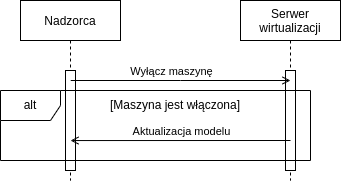
\includegraphics[width=0.6\textwidth]{../diagrams/sequence_diagrams/wylaczenie_maszyny.png}
  \caption{Sekwencja komunikacji wyłączenia maszyny}
  \label{figure:diagrams:sequence_diagrams:wylaczenie_maszyny}
\end{figure}

\end{document}